\section{Prototype}
\label{sec:implementation:prototype}

This section presents the prototype of the Android Wear application developed during the project. \Cref{fig:implementation:prototype:navigation-diagram} shows a navigation diagram of the smart watch application. The letters in the top right corner of the nodes in the diagram references the screenshots shown in \cref{fig:implementation:prototype:screenshots}.

For a list of the supported features in the application, please refer to \cref{sec:implementation:status}.

\begin{figure}[!htb]
    \centering
    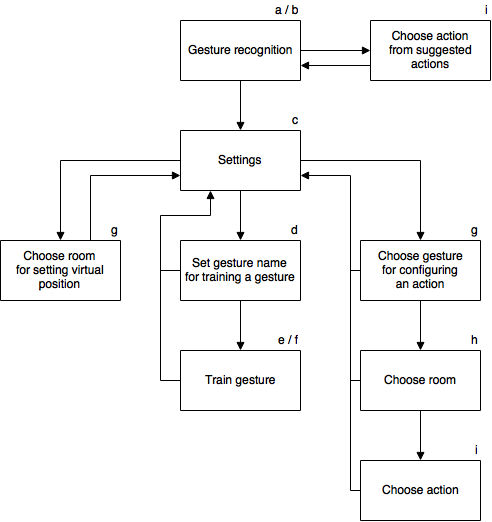
\includegraphics[width=0.7\textwidth]{images/wear-navigation-diagram}
    \caption{Navigation diagram of the application developed for the Android Wear device. Letters in the top right corner of each node refers to the screenshots in figure \cref{fig:implementation:prototype:screenshots}.}
    \label{fig:implementation:prototype:navigation-diagram}
\end{figure}

\begin{figure}[!htb]%
    \centering
    \subbottom[Screen on which the user can start gesture recognition by touching the screen.]{\label{fig:implementation:protoype:}
        \frame{
\includegraphics[width=0.3\textwidth]{images/wear-screenshot-touch-recognize}}
    }
    \subbottom[Screen on which the user can stop gesture recognition by touching the screen. The orange color indicates that recognition has been started.]{\label{fig:implementation:prototype}
        \frame{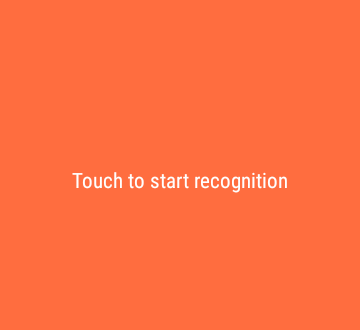
\includegraphics[width=0.3\textwidth]{images/wear-screenshot-recognizing}}
    }
    \subbottom[Settings screen from which the user can set his virtual, train a gesture and configure a new action (create a gesture configuration). When a virtual position is set, the setting can be selected again to unet the virtual position.]{\label{fig:implementation:prototype:}
        \frame{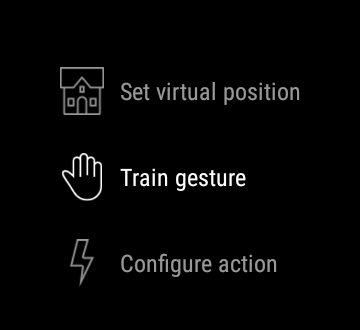
\includegraphics[width=0.3\textwidth]{images/wear-screenshot-settings}}
    }
    \subbottom[Screen shown when the user starts training a gesture. Tapping the ``Gesture name'' button will present the user with a speech recognition interface from which he pronounce the name of the gesture to configure it.]{\label{fig:implementation:protoype:}
        \frame{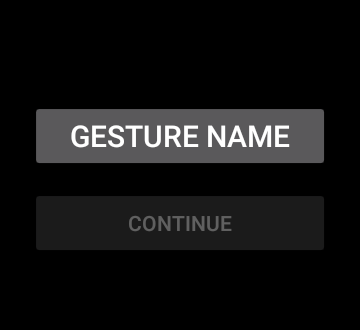
\includegraphics[width=0.3\textwidth]{images/wear-screenshot-name-gesture}}
    }
    \subbottom[Screen shown when training a gesture and the gesture recognizer has not been started. We see that two gesture samples, i.e. gesture templates, have been trained.]{\label{fig:implementation:prototype}
        \frame{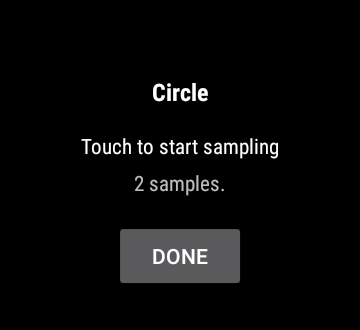
\includegraphics[width=0.3\textwidth]{images/wear-screenshot-touch-train}}
    }
    \subbottom[Screen shown when training a gesture and the gesture recognizer has been started, i.e. the user is performing a gesture.]{\label{fig:implementation:prototype:}
        \frame{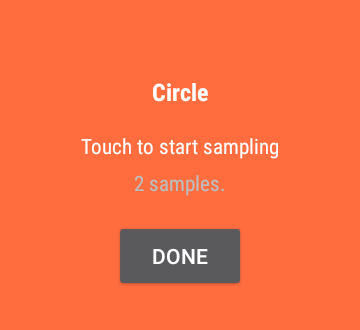
\includegraphics[width=0.3\textwidth]{images/wear-screenshot-training}}
    }
    \subbottom[Gesture picker showing the gestures the user has trained. The gesture picker is used when creating a gesture configuration.]{\label{fig:implementation:protoype:}
        \frame{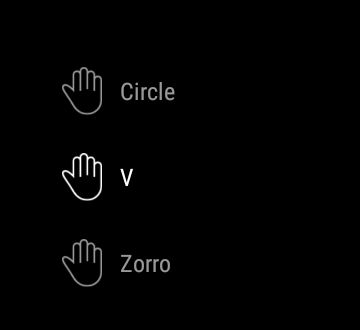
\includegraphics[width=0.3\textwidth]{images/wear-screenshot-gestures}}
    }
    \subbottom[Room picker shown when the user creates a gesture configuration. The picker is also shown when setting a virtual position.]{\label{fig:implementation:prototype}
        \frame{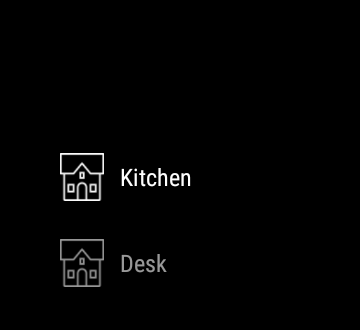
\includegraphics[width=0.3\textwidth]{images/wear-screenshot-rooms}}
    }
    \subbottom[Action picker shown when creating a gesture configuration. A similar picker is shown when the context engine suggests multiple actions.]{\label{fig:implementation:prototype:}
        \frame{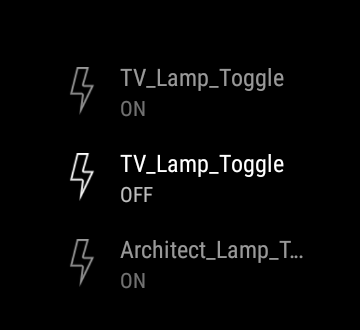
\includegraphics[width=0.3\textwidth]{images/wear-screenshot-actions}}
    }
    \caption{Screenshots of the prototype developed for the Android Wear smart watch.}
    \label{fig:implementation:prototype:screenshots}
\end{figure}

%%% Local Variables:
%%% mode: latex
%%% TeX-master: "../../master"
%%% End:
